\subsection{Entwurf der Applikationsarchitektur}
\label{subsec:entwurf-der-applikationsarchitektur}


Der Entwurf der Applikationsarchitektur bildet die konzeptionelle Grundlage für die technische Umsetzung der entwickelten Web-Applikation.
Das Ziel ist es, eine Struktur zu schaffen, die modular, wartbar und erweiterbar ist, und die gleichzeitig den funktionalen Anforderungen gerecht wird und sich in die bestehende Systemlandschaft integrieren lässt.
Die Architektur der Anwendung ist schichten- und komponentenorientiert aufgebaut und nutzt das Webframework Flask, welches eine klare Trennung zwischen der Präsentations-, Logik- und Datenhaltungsschicht ermöglicht.


\subsubsection{Architekturübersicht}

Die Applikation soll als serverbasierte Webanwendung im Client-Server-Modell funktionieren.
Das bedeutet: Während der Server die Datenverarbeitung, -speicherung und -bereitstellung übernimmt, ermöglicht der Client über den Webbrowser die Darstellung und Interaktion.
Die Anwendung ist in mehrere Schichten gegliedert, zu denen man die einzelnen Programmteile zuordnen kann.
Die Anwendung wird in folgende Schichten gegliedert:

\begin{itemize}
\item Präsentationsschicht (Frontend): Bereitstellung der Benutzeroberfläche über HTML-Templates, CSS und JavaScript.

\item
Applikationslogik (Backend): Implementierung der Geschäftslogik, Steuerung des Datenflusses und Verarbeitung der XML-Dateien.

\item
Datenhaltungsschicht: Persistente Speicherung der extrahierten Mess- und Gerätedaten in einer relationalen Datenbank mittels ORM.

\end{itemize}

Ein schematisches Architekturdiagramm dieser Struktur ist in Abbildung \ref{fig:arch_minimal} dargestellt.

\begin{figure}[H]
    \centering
    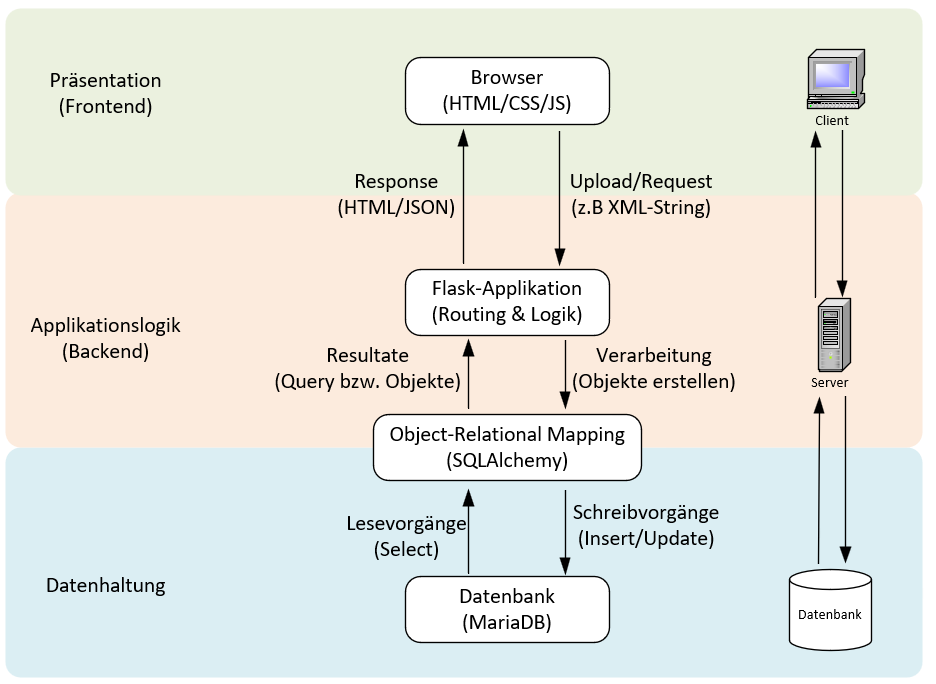
\includegraphics[width=0.95\textwidth]{Grafiken/Architekturdiagramm}
    \caption{schematisches Architekturdiagramm der Applikation}
    \label{fig:arch_minimal}
    {Quelle: Eigene Darstellung mit Microsoft Visio}
\end{figure}

\subsubsection*{Präsentationsschicht}


Die Präsentationsschicht besteht aus einer Kombination aus HTML-Templates und statischen Ressourcen (CSS, JavaScript), die im Verzeichnis templates/ bzw. static/ abgelegt sind.


\begin{itemize}

\item
Die Templates upload.html, reports.html und dut\_report.html bilden die Kernseiten der Weboberfläche.

\item
Statische Dateien wie style.css und dut\_plots.js dienen der Gestaltung und der interaktiven Darstellung von Messergebnissen.

Die Kommunikation mit der Logikschicht erfolgt über die definierten \textit{Flask Blueprints}, die als modulare Controller agieren.

\end{itemize}

\subsubsection*{Applikationslogik}

Die zentrale Geschäftslogik ist in modularen \textit{Blueprints} und \textit{Service-Komponenten} realisiert.

Die drei Blueprints upload, reports und dut kapseln die jeweiligen Funktionsbereiche:

\begin{itemize}

\item
upload: Einlesen und Validieren von XML-Dateien.

\item
dut: Verarbeitung und Anzeige der Daten eines „Device Under Test“.

\item
reports: Zusammenstellung und Ausgabe von Auswertungen.

\end{itemize}

Unterstützt werden diese durch das Modul services/, das die eigentliche Logik zur Datenverarbeitung bereitstellt:

\begin{itemize}

\item
xml\_ingest.py übernimmt das Parsen und Einlesen der XML-Daten.

\item
queries.py enthält vordefinierte Datenbankabfragen.

\item
utils.py und utils\_timeseries.py stellen Hilfsfunktionen zur Verfügung, z. B. zur Zeitreihenanalyse und Datenaufbereitung.

\item
report\_builders.py dient der Erstellung und Formatierung von Report-Daten für die grafische Darstellung.

\end{itemize}

Die Applikationslogik wird über die Datei run.py initialisiert, welche den Flask-Server startet und die Anwendungskonfiguration aus config.py einliest.


\subsubsection*{Datenhaltungsschicht}

Die Datenhaltung erfolgt über ein relationales Datenbanksystem, das über das Flask-eigene \textit{SQLAlchemy ORM} angebunden ist.

Die Datenmodelle sind im Verzeichnis models/ definiert und bilden die logischen Entitäten der Prüfanlage ab, darunter:

\begin{itemize}

\item
dut.py (Device Under Test)

\item
measurement.py (Messdaten)

\item
parameter.py (Prüfparameter)

\item
testbench.py, module.py und ref.py (Referenzdaten und Prüfaufbau)

\end{itemize}

Die Beziehungen zwischen den Modellen ermöglichen eine strukturierte und relationale Abbildung der Prüfdaten, wodurch eine effiziente Abfrage und Analyse möglich ist.

Migrationen werden mit \textit{Alembic} verwaltet, wie das Verzeichnis migrations/ zeigt.


\begin{figure}[H]
    \centering
    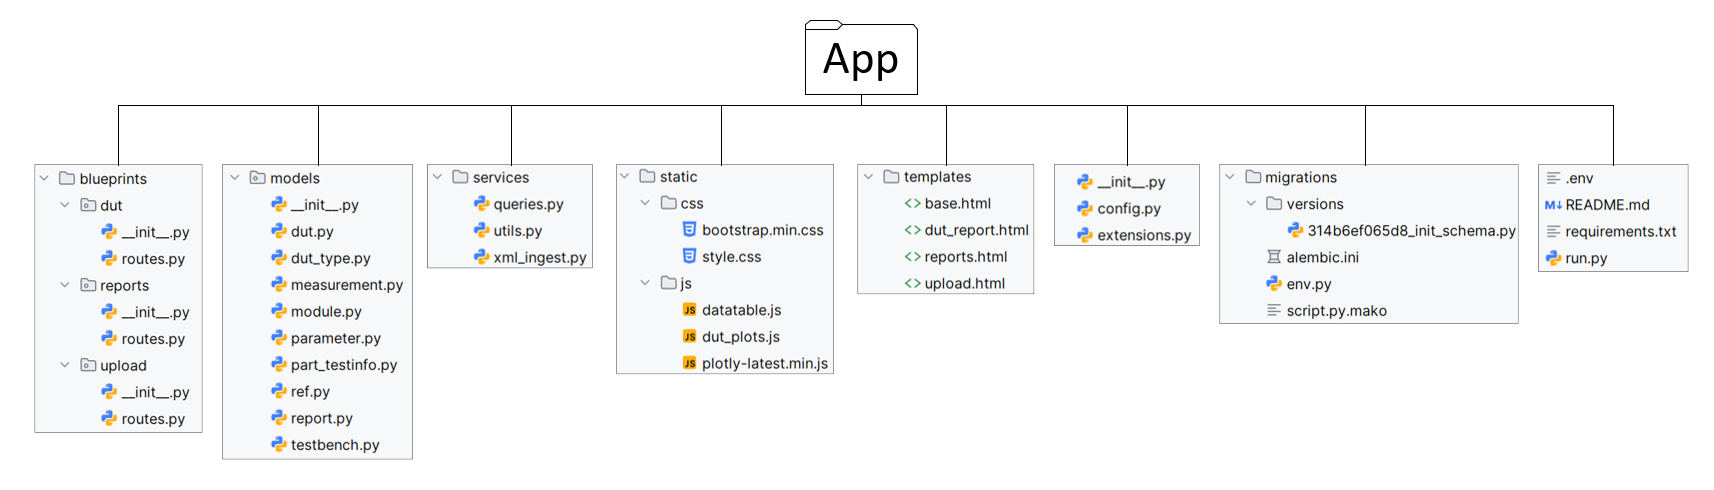
\includegraphics[width=1\textwidth]{Grafiken/Min Ordnerstruktur Projekt}
    \caption{Grundlegende Struktur des Applikations-Ordners}
    \label{fig: Grundlegende Struktur des Applikations-Ordners}
    {Quelle: Eigene Darstellung mit Microsoft Visio}
\end{figure}








